% Copyright 2004 by Till Tantau <tantau@users.sourceforge.net>.
%
% In principle, this file can be redistributed and/or modified under
% the terms of the GNU Public License, version 2.
%
% However, this file is supposed to be a template to be modified
% for your own needs. For this reason, if you use this file as a
% template and not specifically distribute it as part of a another
% package/program, I grant the extra permission to freely copy and
% modify this file as you see fit and even to delete this copyright
% notice. 

\documentclass{beamer}

% There are many different themes available for Beamer. A comprehensive
% list with examples is given here:
% http://deic.uab.es/~iblanes/beamer_gallery/index_by_theme.html
% You can uncomment the themes below if you would like to use a different
% one:
%\usetheme{AnnArbor}
%\usetheme{Antibes}
%\usetheme{Bergen}
%\usetheme{Berkeley}
%\usetheme{Berlin}
%\usetheme{Boadilla}
%\usetheme{boxes}
%\usetheme{CambridgeUS}
%\usetheme{Copenhagen}
%\usetheme{Darmstadt}
%\usetheme{default}
%\usetheme{Frankfurt}
%\usetheme{Goettingen}
%\usetheme{Hannover}
%\usetheme{Ilmenau}
%\usetheme{JuanLesPins}
%\usetheme{Luebeck}
\usetheme{Madrid}
%\usetheme{Malmoe}
%\usetheme{Marburg}
%\usetheme{Montpellier}
%\usetheme{PaloAlto}
%\usetheme{Pittsburgh}
%\usetheme{Rochester}
%\usetheme{Singapore}
%\usetheme{Szeged}
%\usetheme{Warsaw}


% Customize Warsaw color 
\setbeamercolor*{palette primary}{use=structure,fg=white,bg=red!50!black}
\setbeamercolor*{palette secondary}{use=structure,fg=white,bg=red!60!black}
\setbeamercolor*{palette tertiary}{use=structure,fg=white,bg=red!70!black}

% Customize Warsaw block title and background colors
\setbeamercolor{block title}{bg=red!50!black,fg=white}


% List your packages here

\usepackage[colorinlistoftodos]{todonotes}


\title[]{A Generalized Open Source Platform Design for Building Energy Management}

% % A subtitle is optional and this may be deleted
% \subtitle{Product Proposal}

\author[B.~Lauer]{Brian~Lauer\\\and
Advisor: Dr. Suruz Miah}
% - Give the names in the same order as the appear in the paper.
% - Use the \inst{?} command only if the authors have different
%   affiliation.

\institute[Bradley University] % (optional, but mostly needed)
{
  Department of Electrical and Computer Engineering\\
  Bradley University\\
  1501 W. Bradley Avenue\\
  Peoria, IL, 61625, USA
}
% - Use the \inst command only if there are several affiliations.
% - Keep it simple, no one is interested in your street address.

\date[Friday~31,~2020]{Friday, January~31,~2020}
% - Either use conference name or its abbreviation.
% - Not really informative to the audience, more for people (including
%   yourself) who are reading the slides online

\logo{\hfill\href{http://www.bradley.edu}{
\includegraphics[width=0.75cm]{figs/logoBU1-Print}}}  % place logo in every page 


\subject{Mobile Robot Localization}
% This is only inserted into the PDF information catalog. Can be left
% out. 

% If you have a file called "university-logo-filename.xxx", where xxx
% is a graphic format that can be processed by latex or pdflatex,
% resp., then you can add a logo as follows:

% \pgfdeclareimage[height=0.5cm]{university-logo}{university-logo-filename}
% \logo{\pgfuseimage{university-logo}}

% Delete this, if you do not want the table of contents to pop up at
% the beginning of each subsection:
\AtBeginSubsection[]
{
  \begin{frame}<beamer>{Outline}
    \tableofcontents[currentsection,currentsubsection]
  \end{frame}
}




% Let's get started
\begin{document}

\begin{frame}
  \titlepage
\end{frame}

\begin{frame}{Outline}
  \tableofcontents
  % You might wish to add the option [pausesections]
\end{frame}

% Section and subsections will appear in the presentation overview
% and table of contents.
\section{Introduction}

\begin{frame}{Introduction}{}
  % applications of mobile robot navigation and problem descriptio
  	\begin{itemize}
  		\item Residential and commercial buildings account for around 40 \% of energy consumption in US in 2018
  		\item Microgrids which incorporate distributed renewable energy sources will be integrated with smart grids to make energy supply more reliable and decrease costs and transmission losses
  	\end{itemize}
\end{frame}

\begin{frame}{Introduction}{}
\begin{figure}
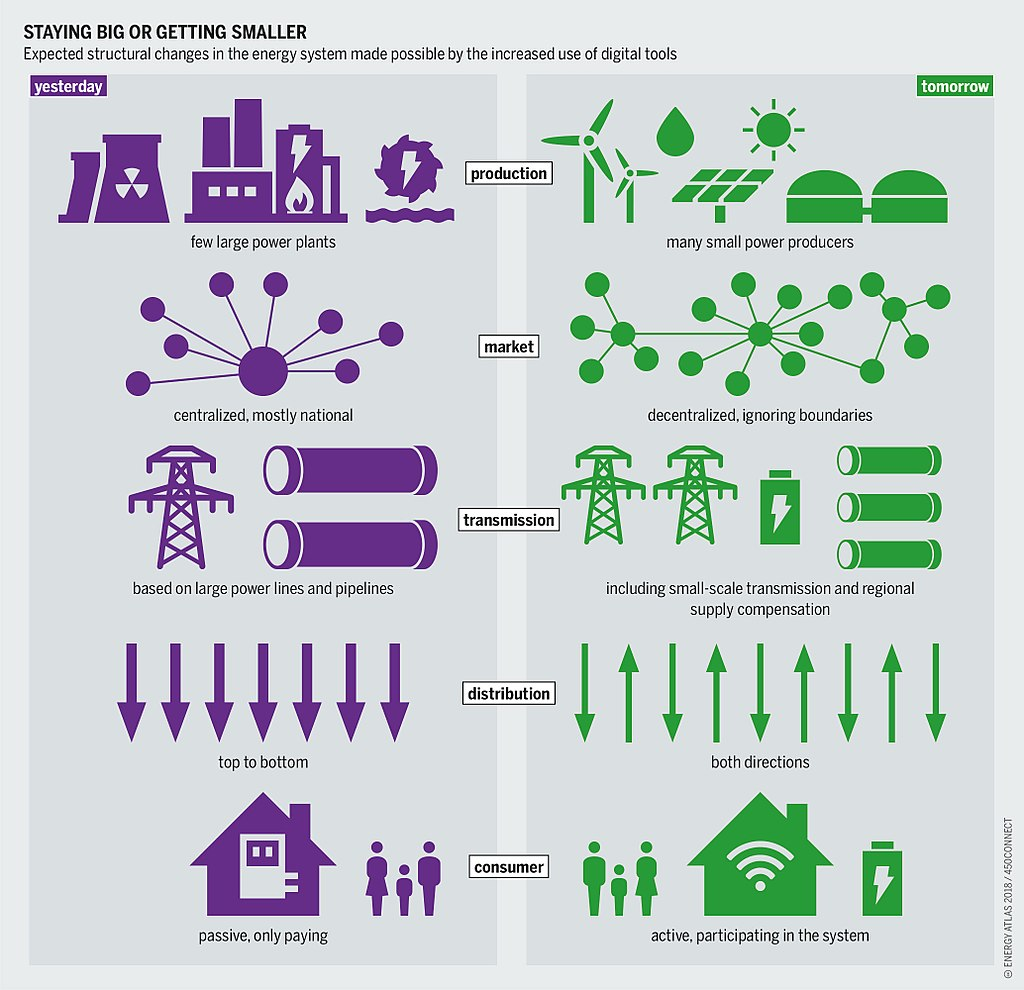
\includegraphics[scale=0.18]{figs/img/microgridsAndSmartgrids}
\caption{Traditional power grid characteristics (left) vs smart grid characteristics (right), courtesy of Wikipedia: \url{https://en.wikipedia.org/wiki/Smart_grid}}
\end{figure}
\end{frame}

\section{Objectives}
\begin{frame}{Objectives}
\begin{enumerate}
\item BEMOSS will be fully analyzed 
\item Prototype of the proposed BEMS will be developed
\item Rotational electromechanical devices will be integrated such as DC motor will be integrated in new platform
\item Determine research avenues - learning, control, estimation algorithms
\item Develop ways to mitigate security threats to reduce power outage costs in the US
\item Deploy the BEMS in community areas to monitor energy costs as well as demonstrate its effectiveness
\end{enumerate}
\end{frame}

\section{Research Approach}
\begin{frame}{Research Approach}
\begin{figure}
\includegraphics[scale=0.35]{figs/ipe/BEMS-SoftwareArchitecture}
\caption{High level software architecture of BEMS}
\end{figure}
\end{frame}

\section{Preliminary Results}
\begin{frame}{Preliminary Results}
\begin{figure}
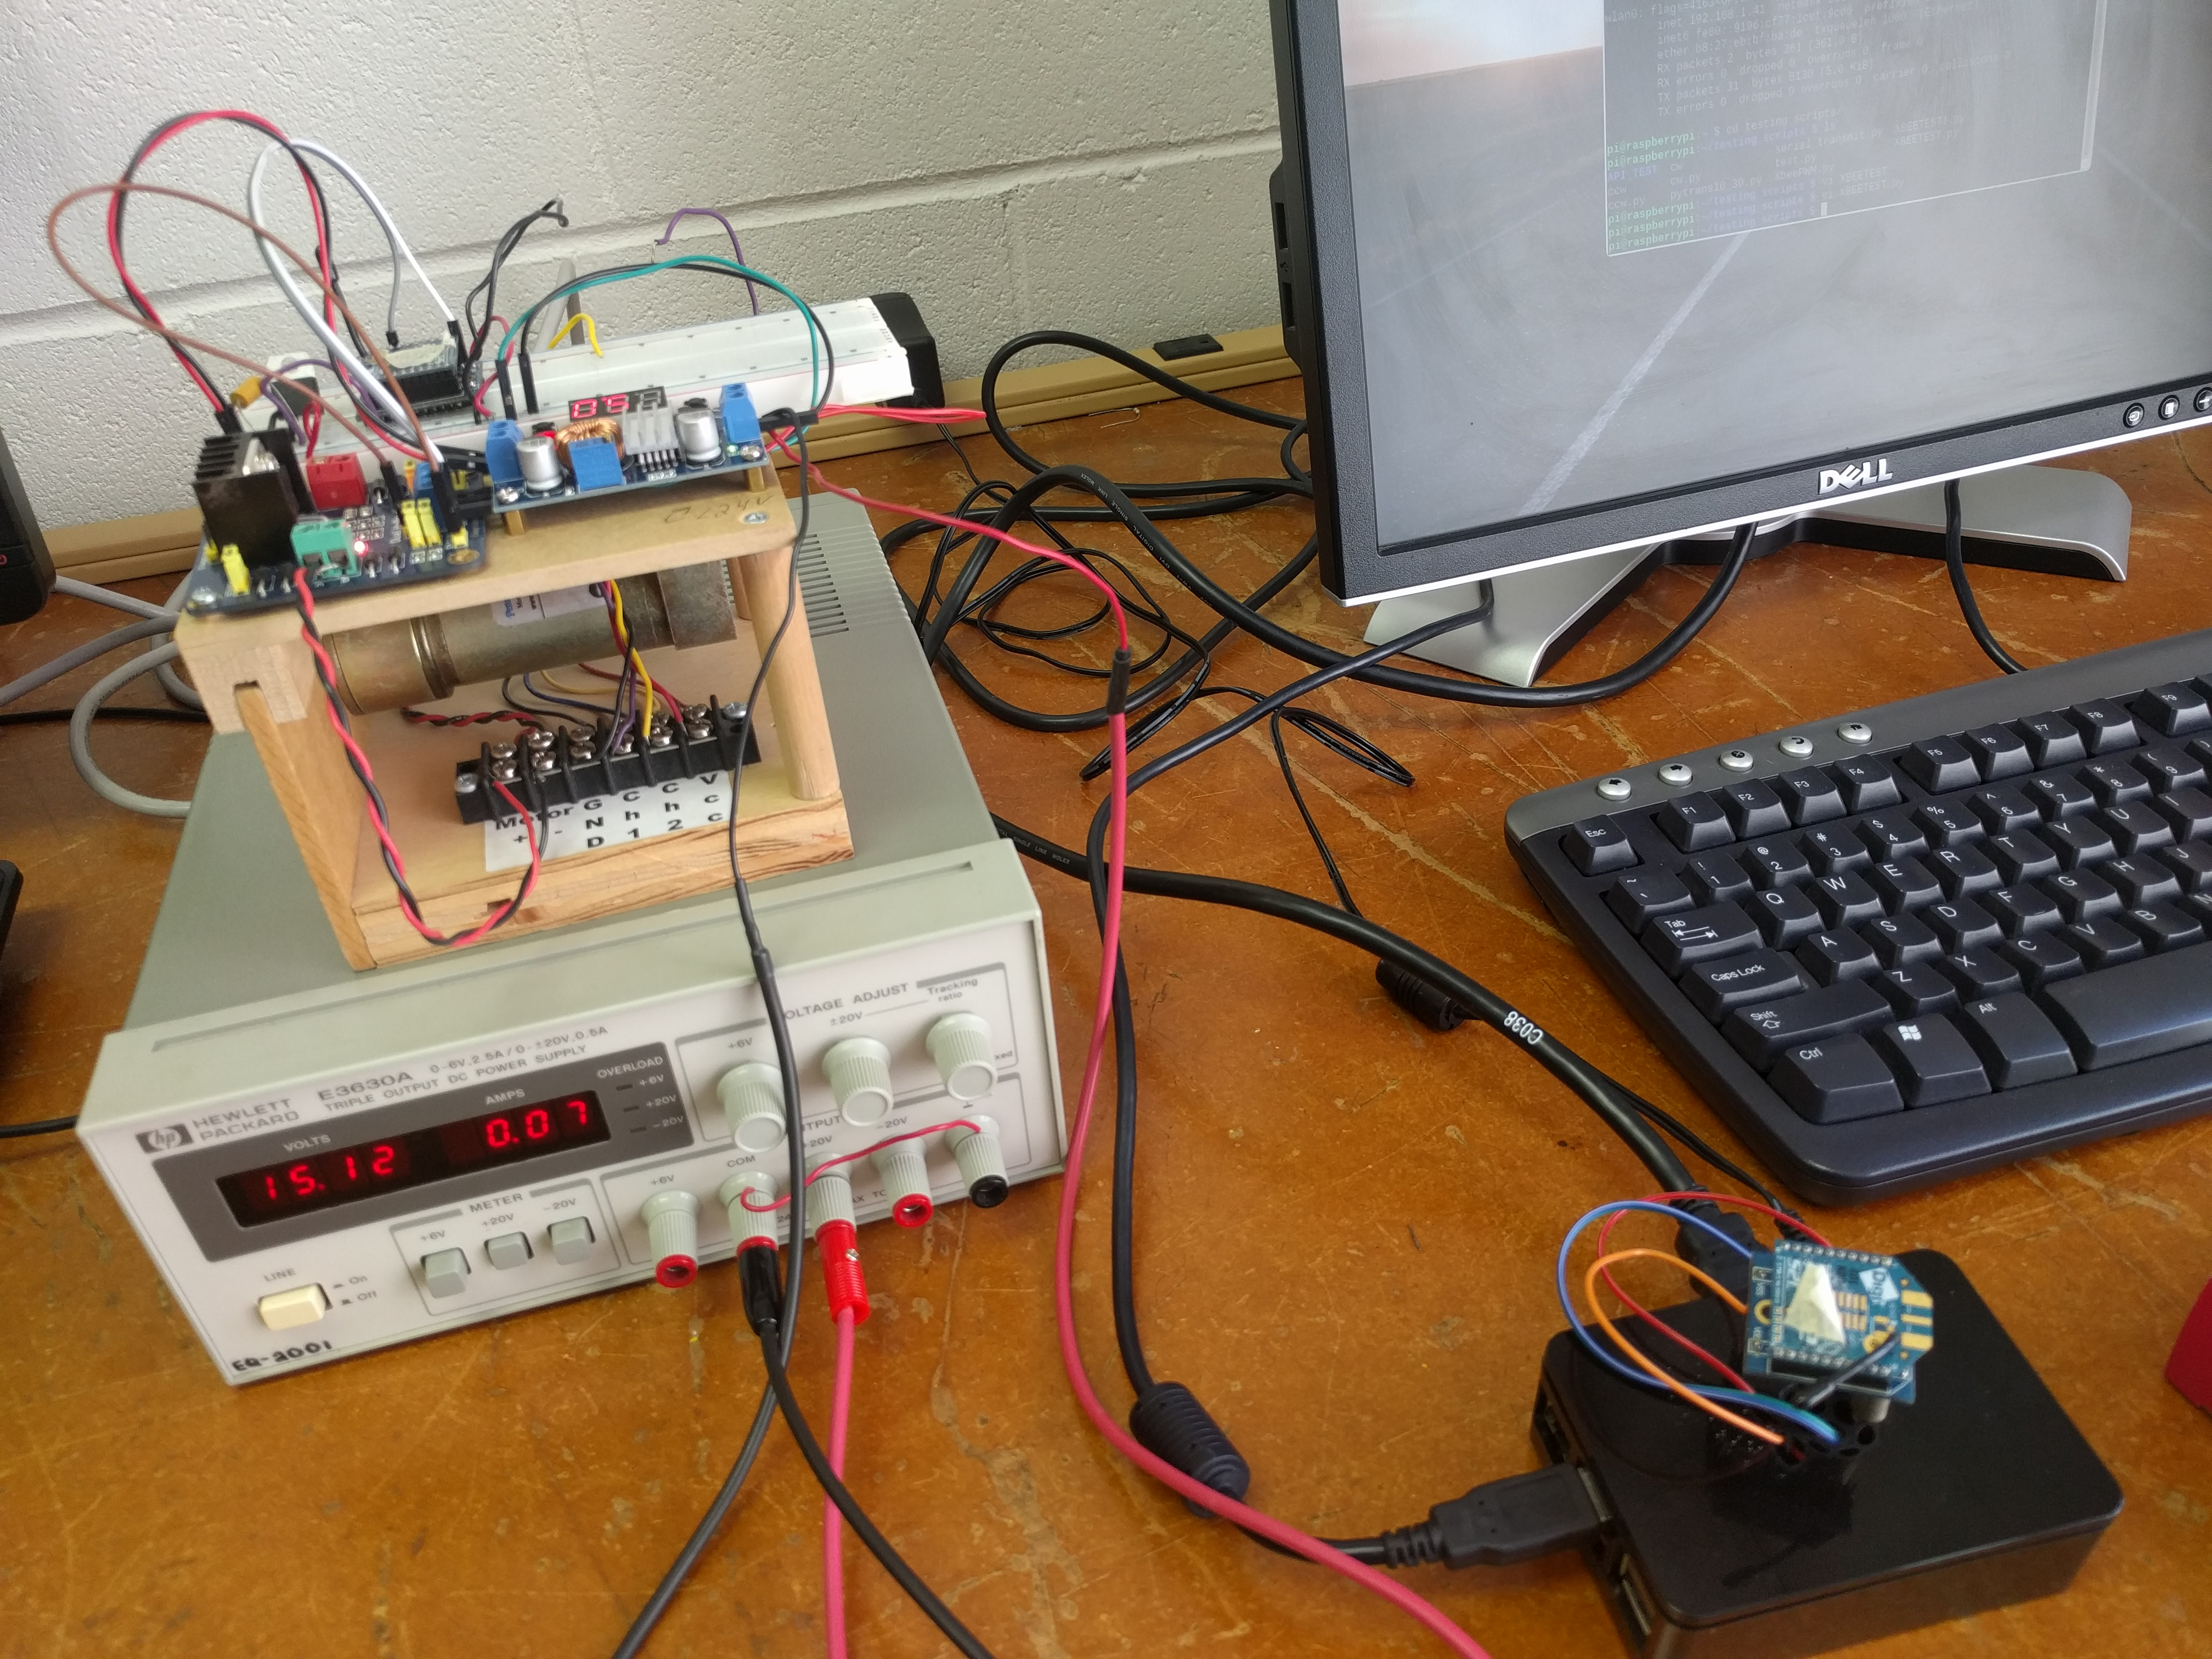
\includegraphics[scale=0.05]{figs/motorSetup.jpg}
\caption{Lab setup of IoT DC motor}
\end{figure}
\end{frame}

\begin{frame}{Preliminary Results}
\begin{figure}
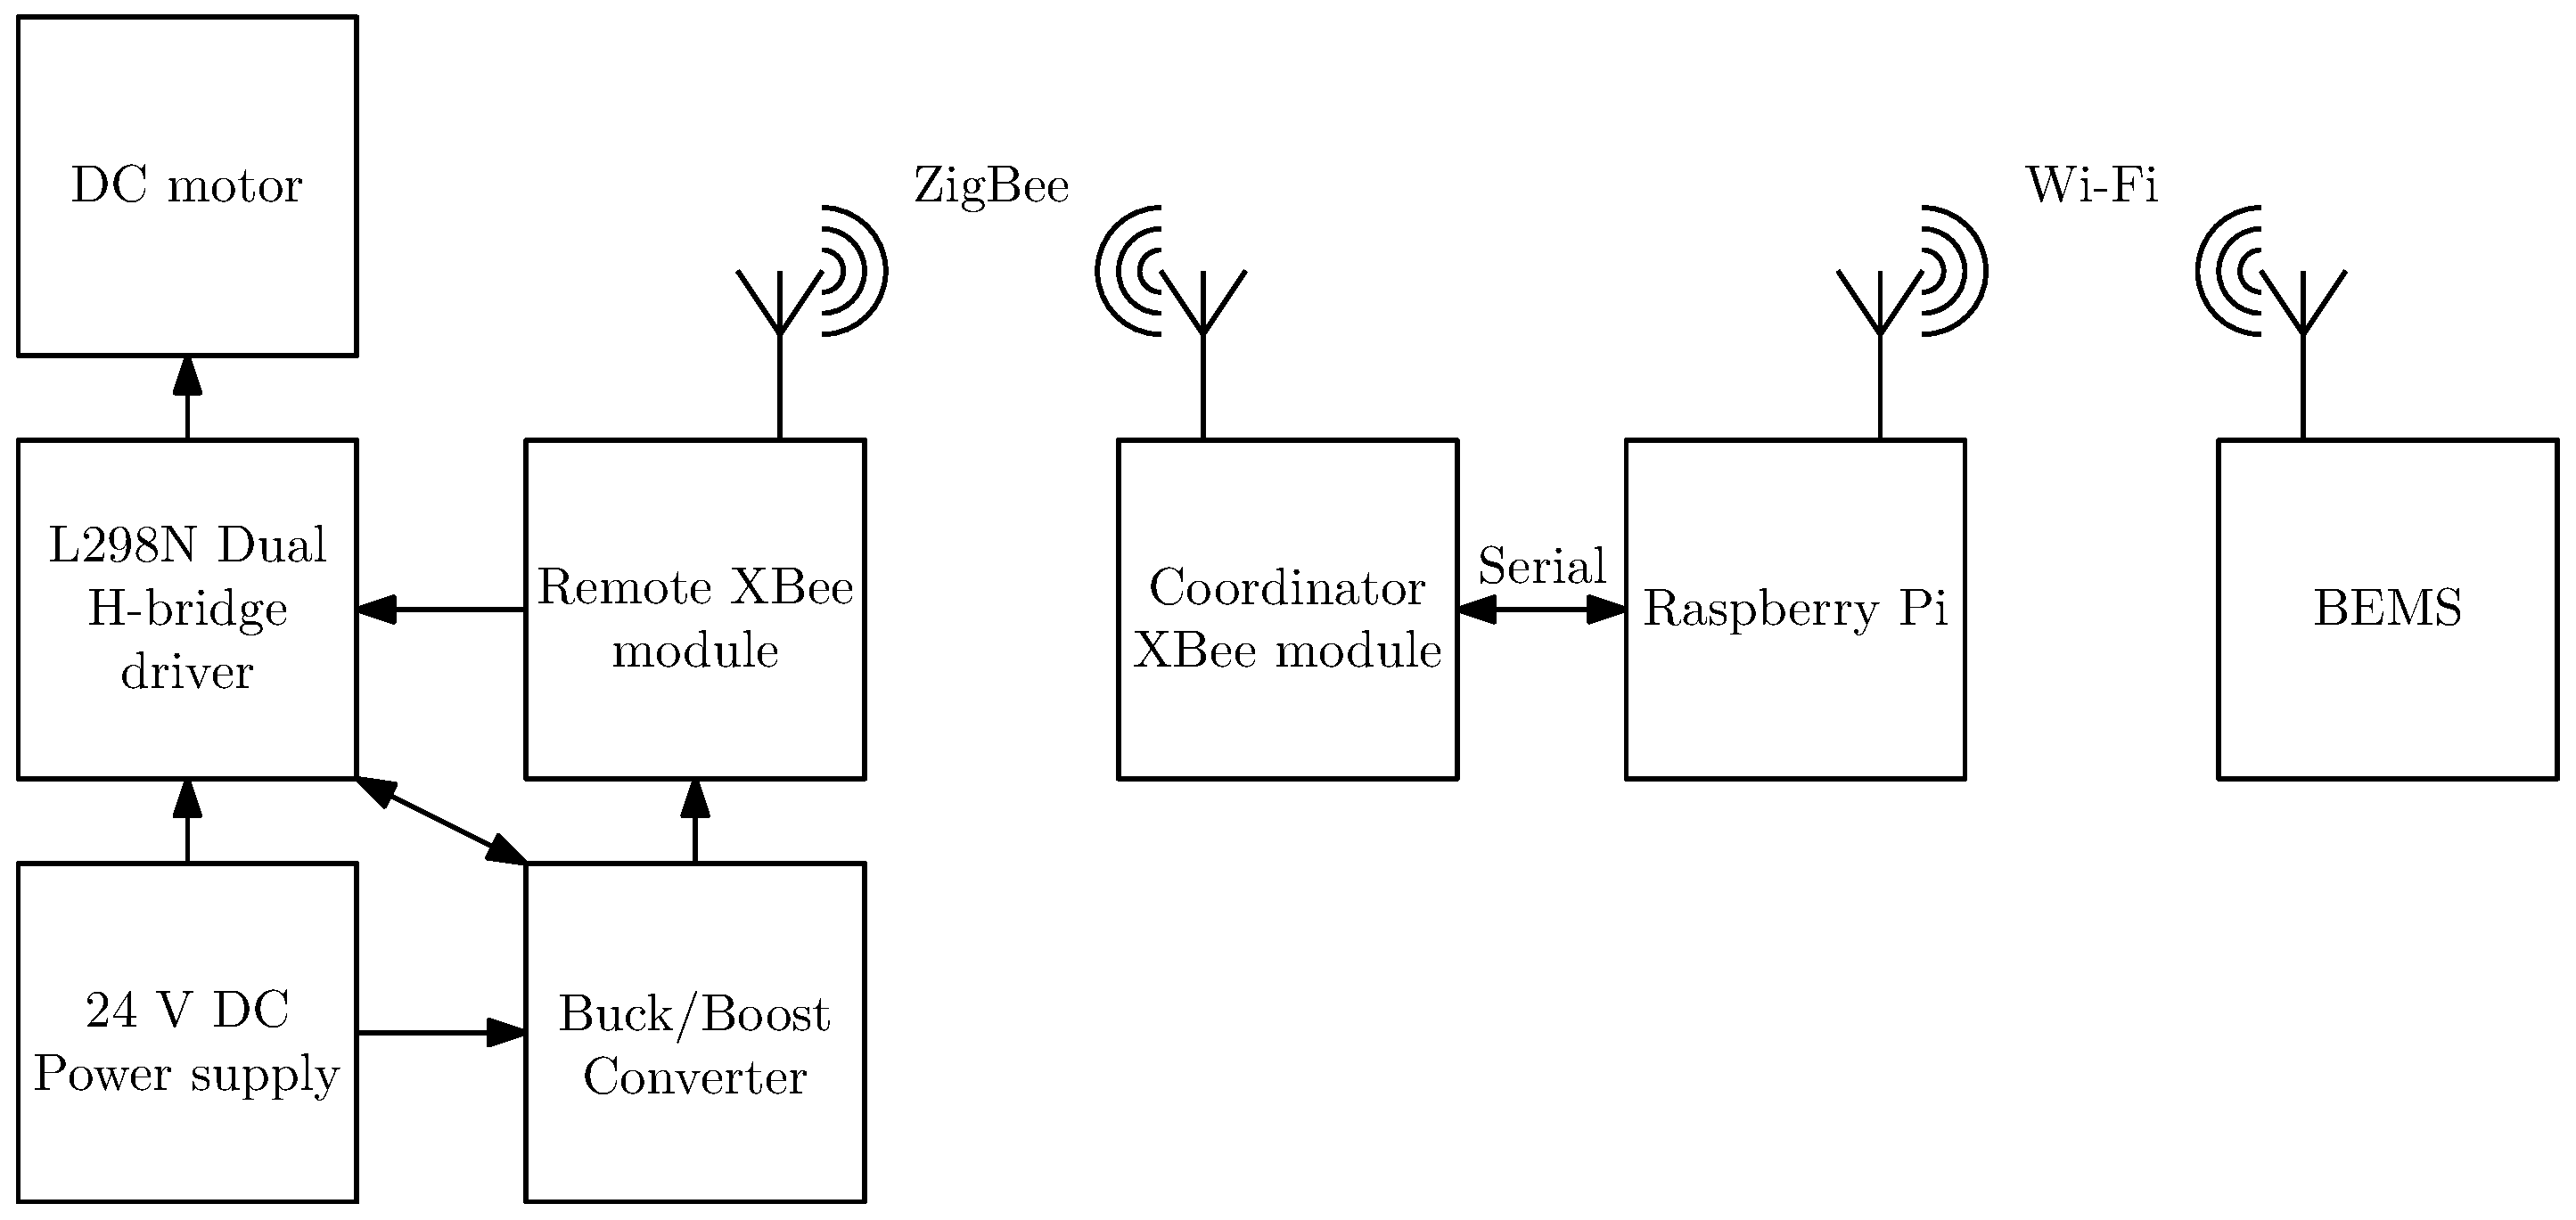
\includegraphics[scale=0.6]{figs/ipe/motorSetup}
\caption{Connection of hardware modules for integrating a IoT device with BEMOSS}
\end{figure}
\end{frame}

\section{Learning, Control, and Estimation Strategies}
\begin{frame}{Learning, Control, and Estimation Strategies}
\begin{itemize}
\item Algorithms will be implemented for solving energy optimization, monitoring, and security problems
\item IoT sensors will be deployed for monitoring voltage and current of different points in the microgrid (state variables)
\item Sensors are vulnerable to cyber attacks 
\item Kalman filter based cyber attack detection scheme will be used
\end{itemize}
\end{frame}

\end{document}



%%% Local Variables:
%%% mode: latex
%%% TeX-master: t
%%% End:
